\section{研究相关理论}
\subsection{排队论}
% 排队现象是在日常生活中经常遇到的一种现象。无论是顾客到商店购买物品,
% 还是病人到医院看病,都可能需要排队等候。这是因为到达服务机构的人数超过了其容量,
% 导致顾客无法立即得到服务。排队现象不仅在个人日常生活中出现,在电话局的占线问题、
% 车站、码头等交通枢纽的车船堵塞和疏导,故障机器的停机待修,水库水量的存储调节等
% 许多场景中也存在。由于顾客到达和服务时间的随机性,因此排队现象几乎是不可避免的。
% 要解决排队问题,增加服务设备可能需要增加投资或发生空闲浪费;但如果服务设备太少,
% 排队现象就会严重,对顾客和社会都会带来不利影响。
排队论是一门应用数学领域的学科,主要研究随机到达、处理和服务的问题。排队论可用于研究各种排队系统,例如超市、银行、工厂生产线等。排队论最早起源于20世纪初的电话系统,现已广泛应用于网络、运输、供应链管理等各个领域。
排队论主要包括三个基本元素:到达过程、服务过程和队列。到达过程是指顾客到达的时间分布;服务过程是指服务时间的分布;队列则是指排队的等待区域。排队论主要关注的是如何通过调整服务设施的数量、服务能力、排队策略等来优化系统性能,从而实现效率最大化、等待时间最小化等目标。
排队论具有很强的实用性,可以帮助企业和组织优化服务流程,提高客户满意度。例如,在银行排队时,排队论可以帮助银行管理者确定柜员数量、窗口开放时间等,从而提高服务效率和客户满意度。排队论还可以用于优化生产线、交通运输系统、网络等各个领域,以提高系统性能。
因此,管理人员必须考虑如何在这两
者之间取得平衡,经常检查目前处理是否得当,研究今后改进对策,以期提高服务质量,降低
成本\cite{ycx, jtgc}。

% 排队模型通常表示为 $X/Y/Z/A/B/C$ 的形式,其中 $X$ 表示相继到达的间隔时间服从的分布,$Y$ 表示服务时间的分布,
% $Z$ 表示服务台的数目,$A$ 表示容量限制,$B$ 表示客源数目,$C$ 表示服务规则。
% 对于公交站台而言,可以将其表示为标准的 $M/M/1$ 模型。该模型具有以下特点:

% 1.输入过程:顾客源是无限的,每个顾客到达的时间相互独立,到达数服从泊松分布,到达过程是平稳的。

% 2.排队规则:单队列,队长没有限制,先到先服务。

% 3.服务机构:单个服务台,每个顾客的服务时间相互独立,
% 服从相同的负指数分布。

% 此外,还假设到达间隔时间和服务时间是相互独立的。

M/M/1排队模型是排队论中的一种简单模型,用于描述一个单一服务通道、
无限容量的队列系统。M表示顾客到达服从泊松分布,即顾客到达服从平均到达率为λ的指数分布;
M表示服务时间服从平均服务率为μ的指数分布;1表示只有一个服务通道。
这个模型可以用于分析单个服务人员在单位时间内完成多少工作,以及顾客在系统中等待的时间。
在这个模型中,每个顾客的到达和服务时间是相互独立的。当一个顾客到达并发现服务台忙时,他会排在队列的末尾等待服务。
顾客在队列中等待的时间是随机的,平均等待时间为Wq=ρ/(μ-λ),其中ρ是系统繁忙率,即平均到达率λ除以平均服务率μ。整个系统的响应时间包括等待时间和服务时间,平均响应时间为W=Wq+1/μ。
这个模型可以用于对不同场景下的队列系统进行分析和优化。例如,在服务速率和到达率相等的情况下,队列将无限制地增长,
这可能会导致服务时间和等待时间都无限增加,因此需要增加服务能力或降低到达率。
已知 $M/M/1$ 模型中到达规律服从参数为 $\lambda$ 的泊松分布,
服务时间服从参数为 $\mu$ 的负指数分布。假设系统中有 $n$ 个顾客,
在 $t$ 时刻状态为 $n$ 的概率为 $P_n(t)$,
则系统的状态方程可以表示为:
\begin{equation}\label{fomula1}
    \begin{cases}
        -\lambda P_0 + \mu P_1 = 0
        \\
       \lambda p_{n - 1} + \mu P_{n + 1} - (\lambda + \mu)P_n = 0 \qquad n\ge 1
       \end{cases}
\end{equation}

公式~\ref{fomula1}~表示关于 $P_n$ 的差分方程,
该方程描述了系统状态之间的转移关系,如图~\ref{fig21}~所示。

\begin{figure}[h]
\centering
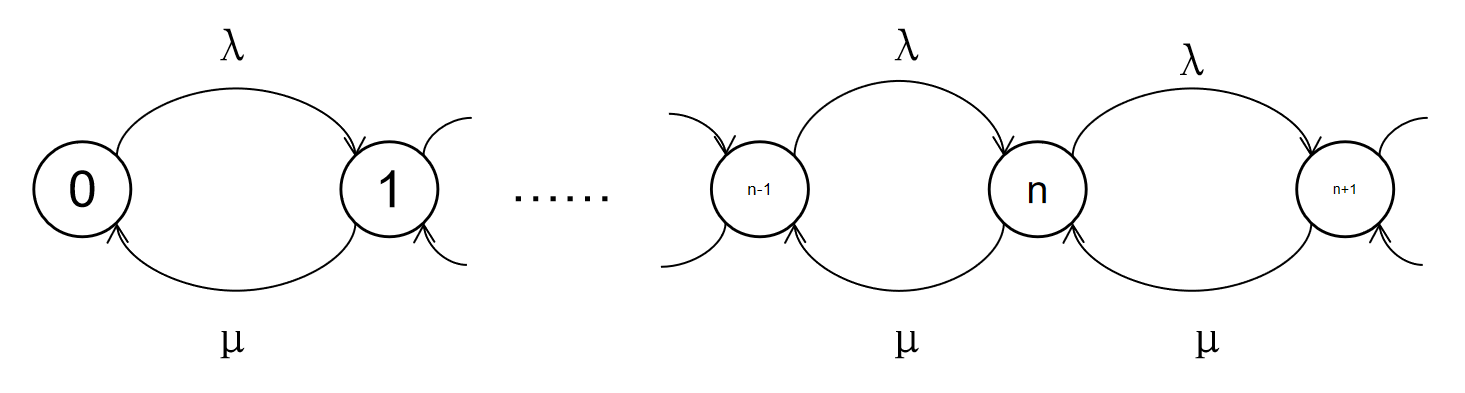
\includegraphics[width=0.80\textwidth]{figs/chap02/fig21.png}
\caption{M/M/1模型状态转移示意图}
\label{fig21}
\end{figure}


要解决排队问题,首先需要收集原始数据,以获得顾客到达间隔和服务时间的经验分布。
然后可以使用统计学方法(例如 $\chi^2$ 检验)确定哪种理论分布最适合数据,并估计其参数值。
常用的分布函数包括泊松分布、负指数分布和爱尔郎分布。
\subsection{运输问题}

经济建设中经常需要解决物资调运问题,即在多个生产基地和消费地点之间制定调运方案,以最小化总运费。
假设有 $m$ 个生产地点 $A_i$,$i=1,2,\dots,m$,每个地点的产量为 $a_i$;有 $n$ 个销地 $B_j$,$j=1,2,\dots,n$,
每个地点的需求量为 $b_j$;从 $A_i$ 到 $B_j$ 运输单位物资的运价为 $c_{ij}$。
我们用 $x_{ij}$ 表示从 $A_i$ 到 $B_j$ 的运量。在产销平衡的条件下,
可以通过求解以下数学模型来得到总运费最小的调运方案:
\begin{equation}\label{fomula2}
    \begin{array}{l} 
        \min z=\sum_{i=1}^{m} \sum_{j=1}^{n} a_{i j} x_{i j} \\
        \left\{\begin{array}{l}
        \sum_{i=1}^{m} x_{i j}=b_{j}, \quad j=1,2, \cdots, n \\
        \sum_{j=1}^{n} x_{i j}=a_{i}, \quad i=1,2, \cdots, m \\
        x_{i j} \geqslant 0
        \end{array}\right.
        \end{array}
\end{equation}

式~\ref{fomula2}~描述了一个产销平衡的运输问题,包含 $m \times n$ 个变量和 $m+n$ 个约束方程。但是,由于存在一些关系式,如:
$$\sum_{j=1}^{n} b_j = \sum_{i = 1}^{m} \left ( \sum_{j=1}^{n} \right ) = \sum_{j=1}^{n} \left ( \sum_{i=1}^{m} \right ) = \sum_{i=1}^{m} a_i$$

这些关系式使得模型的独立约束方程最多只有 $m+n-1$ 个,从而简化了求解运输问题的计算。因此,通常可以采用表上作业法来解决这类问题。

\subsection{线性规划}
生产管理和经营活动中常提出如何合理利用有限资源以达到最佳经济效益的问题,这类问题的解决引出了线性规划。
线性规划问题的形式各异,因此需要将各种数学模型转换为标准形式。规定的标准型式为:
$$\begin{aligned}
    & \max z =\sum_{j=1}^{n} c_{j} x_{j} \\
    & \left\{\begin{array}{l}
    \sum_{j=1}^{n} a_{i j} x_{j}=b_{i}, \quad i=1,2, \cdots, m \\
    x_{j} \geqslant 0, \quad j=1,2, \cdots, n
    \end{array}\right.
    \end{aligned}$$

    在实际数值计算中,更常用的是线性规划的矩阵形式:
$$
\begin{aligned}
    &max z=CX \\
    &AX = b\\
    &X \ge 0
\end{aligned}
$$

其中:\\
$$
\begin{pmatrix}
    a_{11}  & a_{12} &… &a_{1n} \\
     … &  …& &…\\
     a_{m1} & a_{m2} &…&a_{mn}
    \end{pmatrix}=\left ( P_1,P_2,…,P_n \right ) 
    ;0=\begin{bmatrix}
     0\\
     0\\
     …\\
    0
\end{bmatrix}
$$



A——约束条件的 $x \times n$ 维系数矩阵,一般 $m < n$;

b——资源向量;

C——价值向量

X——决策变量向量。


% \subsection{动态规划}
% 在生产和科学实验中,存在一类过程需要分为若干个互相关联的阶段进行决策,
% 以达到最佳效果。因此,各个阶段的决策不能任意确定,
% 而是取决于当前的状态并影响后续的发展。确定各个阶段的决策后,就可以形成一个决策序列,
% 从而决定整个过程的活动路径。这种问题被称为多阶段决策过程或序贯决策过程,
% 因其前后关联具有链状结构,如图~\ref{fig22}~所示。
% \begin{figure}[h]
%     \centering
%     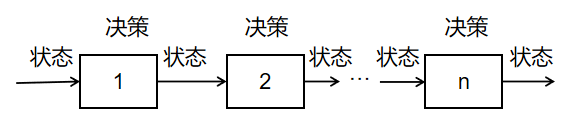
\includegraphics[width=0.80\textwidth]{figs/chap02/dp.png}
%     \caption{多阶段决策示意图}
%     \label{fig22}
% \end{figure}


% 多阶段决策问题中,各阶段的决策往往随时间变化,依赖于当前状态并引起状态转移。
% 因此,所得决策序列具有“动态”的特性,因而称其处理方法为动态规划方法。

% \subsection{图与网络模型}
% 图论是一种广泛应用于各个领域的运筹学分支,
% 可以应用于物理学、化学、控制论、信息论、科学管理、电子计算机等领域。
% 实际生活、生产和科学研究中有许多问题可以使用图论理论和方法解决。例如,运输系统的设计,再例如,各种通信网
% 络的合理架设,交通网络的合理分布等问题,应用图论的方法求解都很简便\cite{gycx}。

% \subsection{对策论}
% 对策论亦称竞赛论或博弈论,是研究具有斗争或竞争性质现象的数学理论和方法。
% 一般认为,它是现代数学的一个新分支,是运筹学的一个重要学科。对策论发展的历史并
% 不长,但由于它研究的问题与政治、经济、军事活动乃至一般的日常生活等有着密切联系,
% 并且处理问题的方法具有明显特色,所以日益引起广泛注意。
% 对策问题本质上都由三个要素组成:

% 1.局中人——在一个对策行为(或一局对策)中, 有权决定自己行动方案的对策参加者, 称为局中
% 人。通常用 $I$ 表示局中人的集合。

% 2.策略集——一局对策中,可供局中人选择的一个实际可行的完整的行动方案称为一个策略。参
% 加对策的每一局中人 $i$ , $i \in I$ 都有自己的策略集 $S_i$ 。

% 3.赢得函数——在一局对策中,各局中人选定的策略形成的策略组称为一个局势,即若 $S_i$ 是第 $i$ 个局中人的一个策略,则 $n$ 个局中人的策略组
% $$
% s = \left(s_1,s_2,…,s_n\right)
% $$
% 就是一个局势。对任一局势 $s \in S$ ,局中人 $i$ 可以得到一个赢得函数 $H_i(s)$

\subsection{整数规划}
% 在线性规划问题中,有些最优解可能是分数或小数,对于某些具体问
% 题,常有要求解答必须是整数的情形(称为整数解)。例如,所求解是机器的台数、完成工
% 作的人数或装货的车数等,分数或小数的解答就不合要求。为了得到可行的整数最优解,需要另行研究。
% 称这样的问题为整数规划(integer programming)。
% 整数规划是最近几十年来发展起来的规划论中的一个分支。
% 整数规划中如果所有的变数都限制为(非负)整数,就称为纯整数规划(pure integer programming)或称为全整数规划(all intege r programming); 如果仅一部分变数限制为整
% 数,则称为混合整数计划(mixed integer programming)。

在线性规划中,有时最优解可能是分数或小数,但有些问题要求解必须是整数,
例如机器台数、工人人数或车辆数等。为了得到可行的整数最优解,
需要研究整数规划。整数规划是最近几十年中发展起来的规划论分支,其中,
所有变量都限制为整数的问题被称为纯整数规划或全整数规划,
而仅有一部分变量限制为整数的问题则称为混合整数计划。
整数规划的应用广泛,可用于生产、管理、科学研究等各个领域。

\subsection{线性目标规划}
在实际情况下会产生多目标问题,如在运输问题中,可能同时需要尽量减少运输成本,减少稀缺资源的消耗,减少运输时间。
目标规划是解决存在多个目标的最优化问题的方法,它把多目标决策问题转化为线性规划问题来求解\cite{gycx}。

\subsection{VSP问题}
% 车辆调度问题(vehicle scheduling problem, VSP)是由 Dantzig 和 Ramser 于 1959 年
% 提出的,虽经多人潜心研究,但由于其复杂性大,目前仍未找到多项式算法,现有研究多把精力集中于研究高质量的启发式算法方面。
% 启发式方法是寻求解决问题的一种方法和策略;它也可以是面向某种具体问题的一种求解方法。它建立在人们经验和判断的基础之上,
% 体现了人的主观能动作用和创造力。

% VSP问题的常规形式一般指:对一系列发货点和收货点,组织适当的行车路线,使车
% 辆有序地通过它们,在满足一定的约束条件下(例如货物需求量与发送量、交发货时间、车
% 量容量限制、行驶里程限制、行驶时间限制等),力争实现一定的目标(如空驶里程最短,运
% 输费用极小,车辆按时到达,使用车辆数量尽可能少等)。车辆调度问题的分类法很多,
% 例如可根据车辆满载与否分为满载问题与非满载问题,
% 根据可用车场数分为单车场问题与多车场问题,根据可用车辆的车型数分为单车型问题
% 与多车型问题,根据决策者的要求分为单目标问题与多目标问题等。

车辆调度问题(VSP)是一项由Dantzig和Ramser于1959年提出的挑战性问题,虽然经过多年的研究,
但由于其复杂性较高,至今仍未找到多项式时间算法,因此目前的研究主要集中于高质量的启发式算法。
启发式算法是一种解决问题的策略和方法,建立在人们的经验和判断基础上,反映了人的主观能动作用和创造力。

通常情况下,VSP问题的常规形式是指:在满足各种约束条件(如货物需求量与发送量、交发货时间、车辆容量限制、
行驶里程限制、行驶时间限制等)的情况下,有序地组织车辆行驶路线,以实现某些目标(如最小化空驶里程、
最小化运输费用、确保车辆按时到达、尽可能减少使用车辆数量等)。根据不同的约束条件和目标,
VSP问题可被分类为满载问题和非满载问题、单车场问题和多车场问题、单车型问题和多车型问题、
单目标问题和多目标问题等。
% \subsection{离散时间模拟包SimPy}

% SimPy是一个用Python编写的基于进程的离散事件模拟框架。
% 使用SimPy,可以使用Python生成器函数定义模拟流程,例如对客户、
% 车辆等活动组件进行建模。此外,SimPy还支持模拟各种类型的共享资源,
% 例如服务器、结账柜台和隧道,以便对有限容量的瓶颈进行建模。

% \subsection{开源软件包Pyomo}
% Pyomo是一个基于Python的开源软件包,用于创建和分析优化模型,支持多种优化功能。Pyomo可用于定义符号问题并创建具体的实例,使用标准解决程序解决这些实例。Pyomo支持多种问题类型,包括线性规划、二次规划、非线性规划和整数线性规划。此外,Pyomo支持全功能编程语言中的分析和脚本编写。除此之外,Pyomo还提供了开发高级优化和分析工具的有效框架。例如,PySP包提供了通用的随机规划求解程序,它利用了Pyomo的建模对象嵌入在功能全面的高级编程语言中的事实,这种语言允许使用Python并行通信库透明地并行化子问题。

% \subsection{数学规划优化系统Gurobi}
% Gurobi是美国 Gurobi Optimization 公司开发的下一代大规模优化器。
% 它已被证明在生产、金融、保险、交通、服务等领域中能够处理复杂和庞大的问题,为决策提供高质量的保障。
% 在理论和实践中,Gurobi优化工具一直被证明是性能领先的大规模优化器。